\documentclass{article}

\usepackage[utf8]{inputenc}
\usepackage[T1]{fontenc}
\usepackage[francais]{babel}
\usepackage{url}
\usepackage{color}
\usepackage{verbatim}
\usepackage{amsmath,amssymb,amsfonts}
\usepackage{graphicx}
\usepackage[french]{algorithm2e}
\usepackage{geometry}
\usepackage{caption}
\captionsetup[figure]{slc=on}
\usepackage{enumitem}
\usepackage{listings}
\usepackage{listingsutf8}
\frenchbsetup{StandardLists=true}
\usepackage{mcode}
\lstset{language=matlab}
\lstset{
	breaklines=true, 
	showspaces=false, 
	keepspaces=true, 
	numbers=left, 
	frame=shadowbox, 
	keywordstyle=\color{blue},
	basicstyle=\ttfamily\small,
	commentstyle=\color{green}
}
\geometry{hmargin=2.5cm, vmargin=2.5cm}

\title{\textbf{Traitement d'images TP4 : Détection de contour}}
\author{Line \bsc{POUVARET}, Hamdi \bsc{BENAOUN}}
\date{2015-2016}

\begin{document}
\maketitle

\section*{2. Dérivation par simples différences finies}
\subsection*{2.1 Filtre de Roberts}
\begin{itemize}\renewcommand{\labelitemi}{$\bullet$}
	\item Fonction roberts\_differential, dans MatLab :
	
\begin{lstlisting}
pic_x = conv2(pic, D, 'same');
pic_y = conv2(pic, D', 'same');
\end{lstlisting}

	\item calcul de la norme, dans MatLab :
\begin{lstlisting}
pic_norm = sqrt(power(pic_x, 2)+power(pic_y, 2));
\end{lstlisting}
	\item Images des gradients en x, y et de la norme :
	
\begin{center}
\fbox{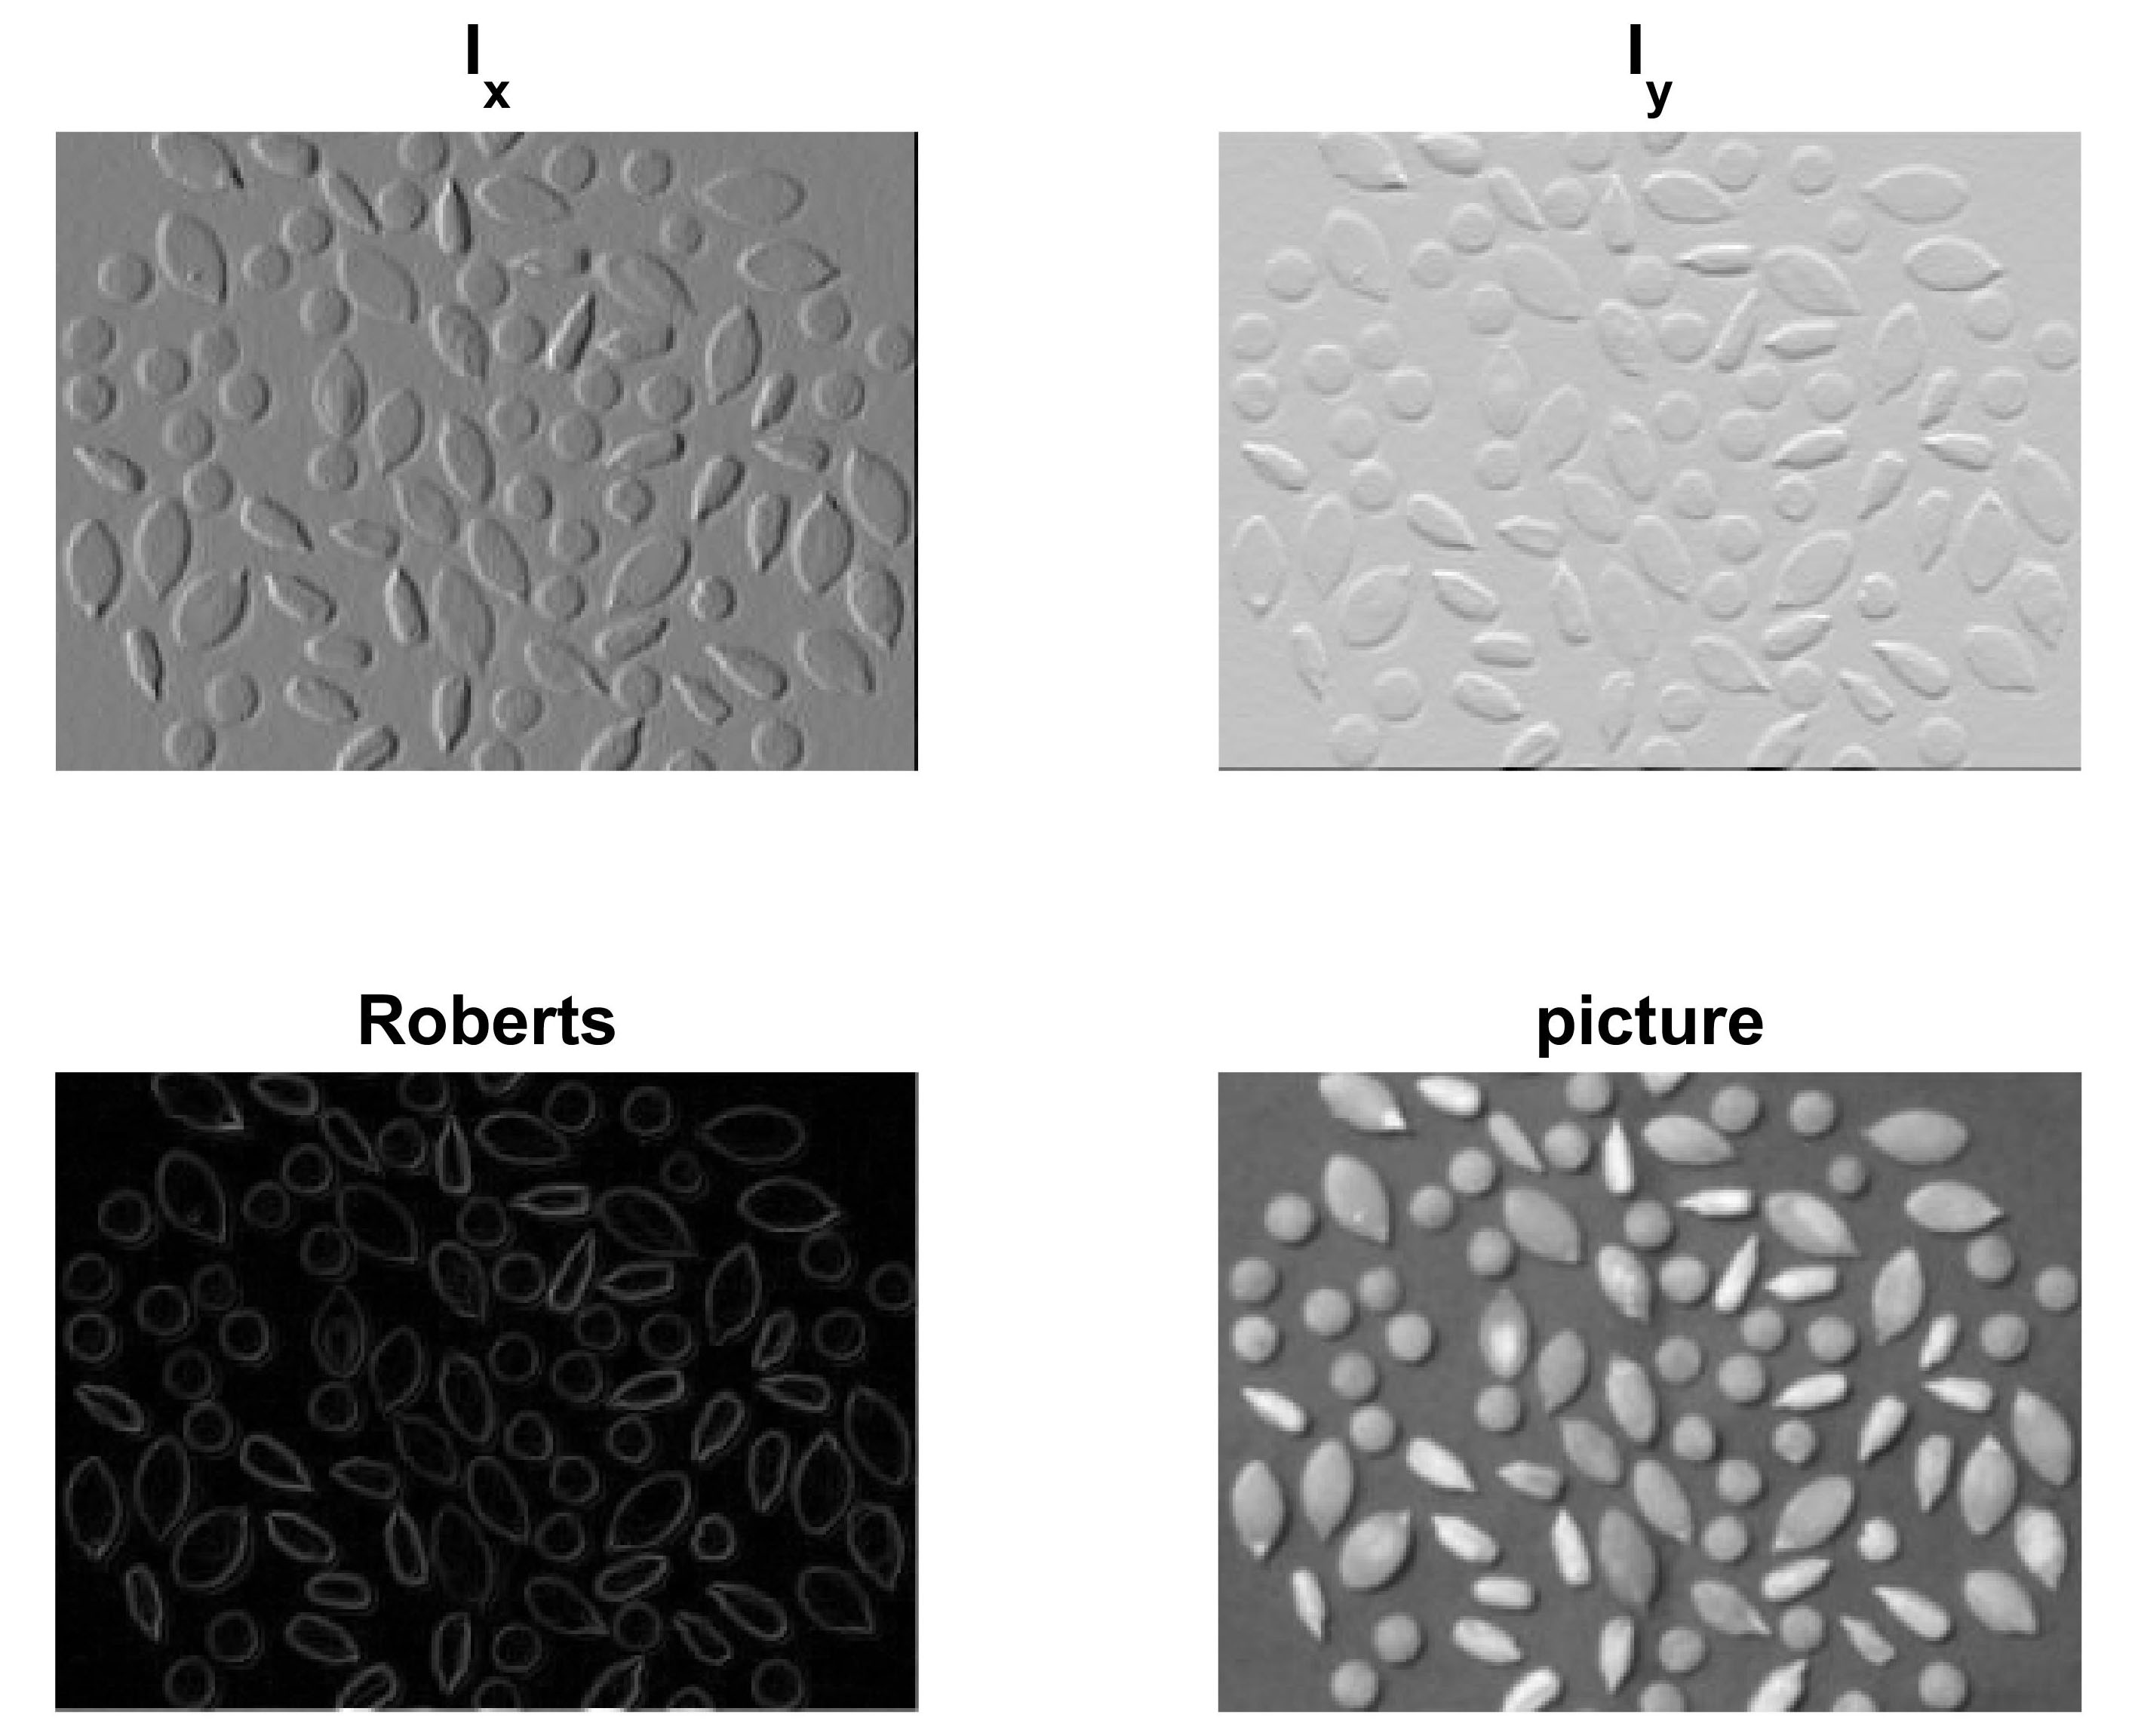
\includegraphics[width=10cm]{gradients_norme_graines.jpg}}
\end{center}

Le gradient en x prend des valeurs qui varient de -98 à 98.

Le gradient en y prend des valeurs qui varient de -232 à 73.

La norme prend des valeurs qui varient de 0 à 232.\\

On remarque au niveau de l'image de la norme, que certaines ombres des graines sont détectés comme des contours (c'est logique puisqu'il y a une variation du sombre au clair).

\end{itemize}

\subsection*{2.2 Filtre de Sobel}

\begin{itemize}\renewcommand{\labelitemi}{$\bullet$}
	\item Fonction sobel\_differential dans MatLab :
	
\begin{lstlisting}
S=[1,2,1];
D=[1,0,-1];
Gx=S'*D;
Gy=D'*S;

pic_x = conv2(pic, (1/4)*Gx,'same');
pic_y = conv2(pic, (1/4)*Gy, 'same');

pic_norm = sqrt(power(pic_x, 2)+power(pic_y, 2));
\end{lstlisting}

	\item Images des gradients en x, y et de la norme :

\begin{center}
\fbox{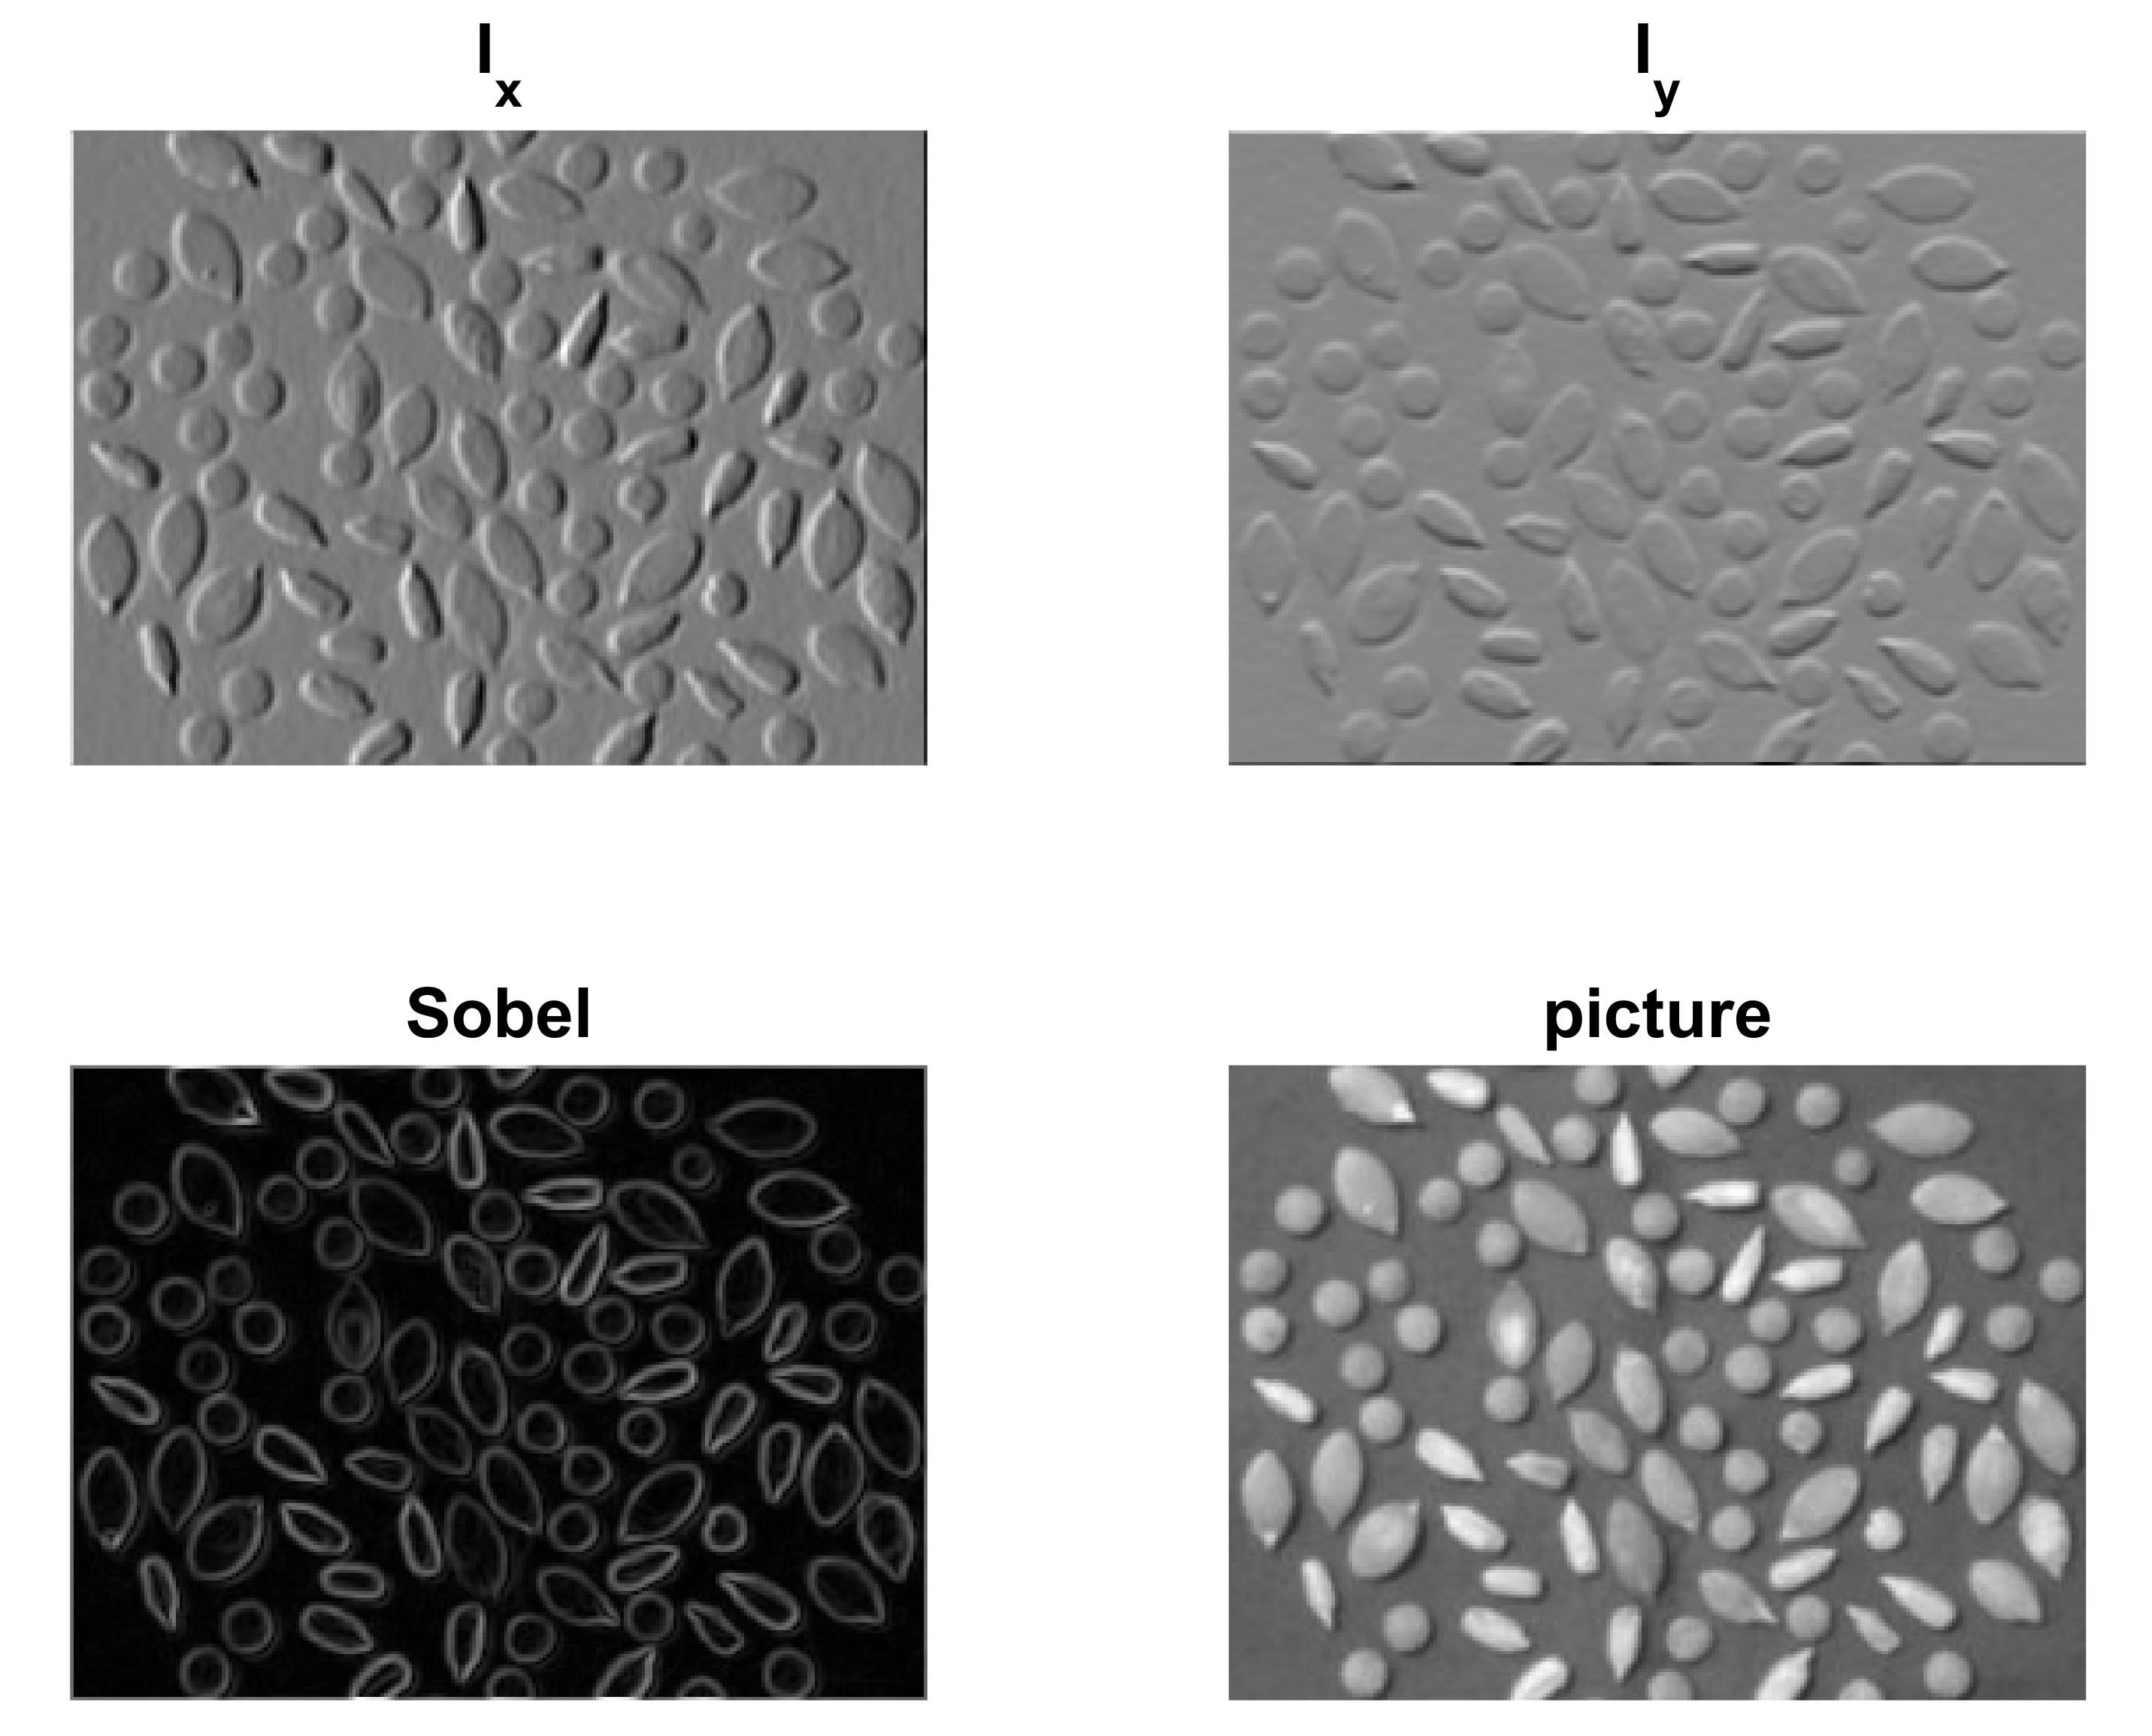
\includegraphics[width=10cm]{gradients_norme_sobel.jpg}}
\end{center}

Les vrais contours des graines sont beaucoup plus nets. On constate tout de même encore un peu les ombres qui ont été détectées mais elles sont beaucoup moins visibles.
\end{itemize}

\subsection*{2.3 Ajout d'un bruit gaussien}
On ajoute un bruit gaussien avec RSB = 10db.
\begin{itemize}\renewcommand{\labelitemi}{$\bullet$}
	\item Avec le filtre de Roberts :

\begin{center}
\fbox{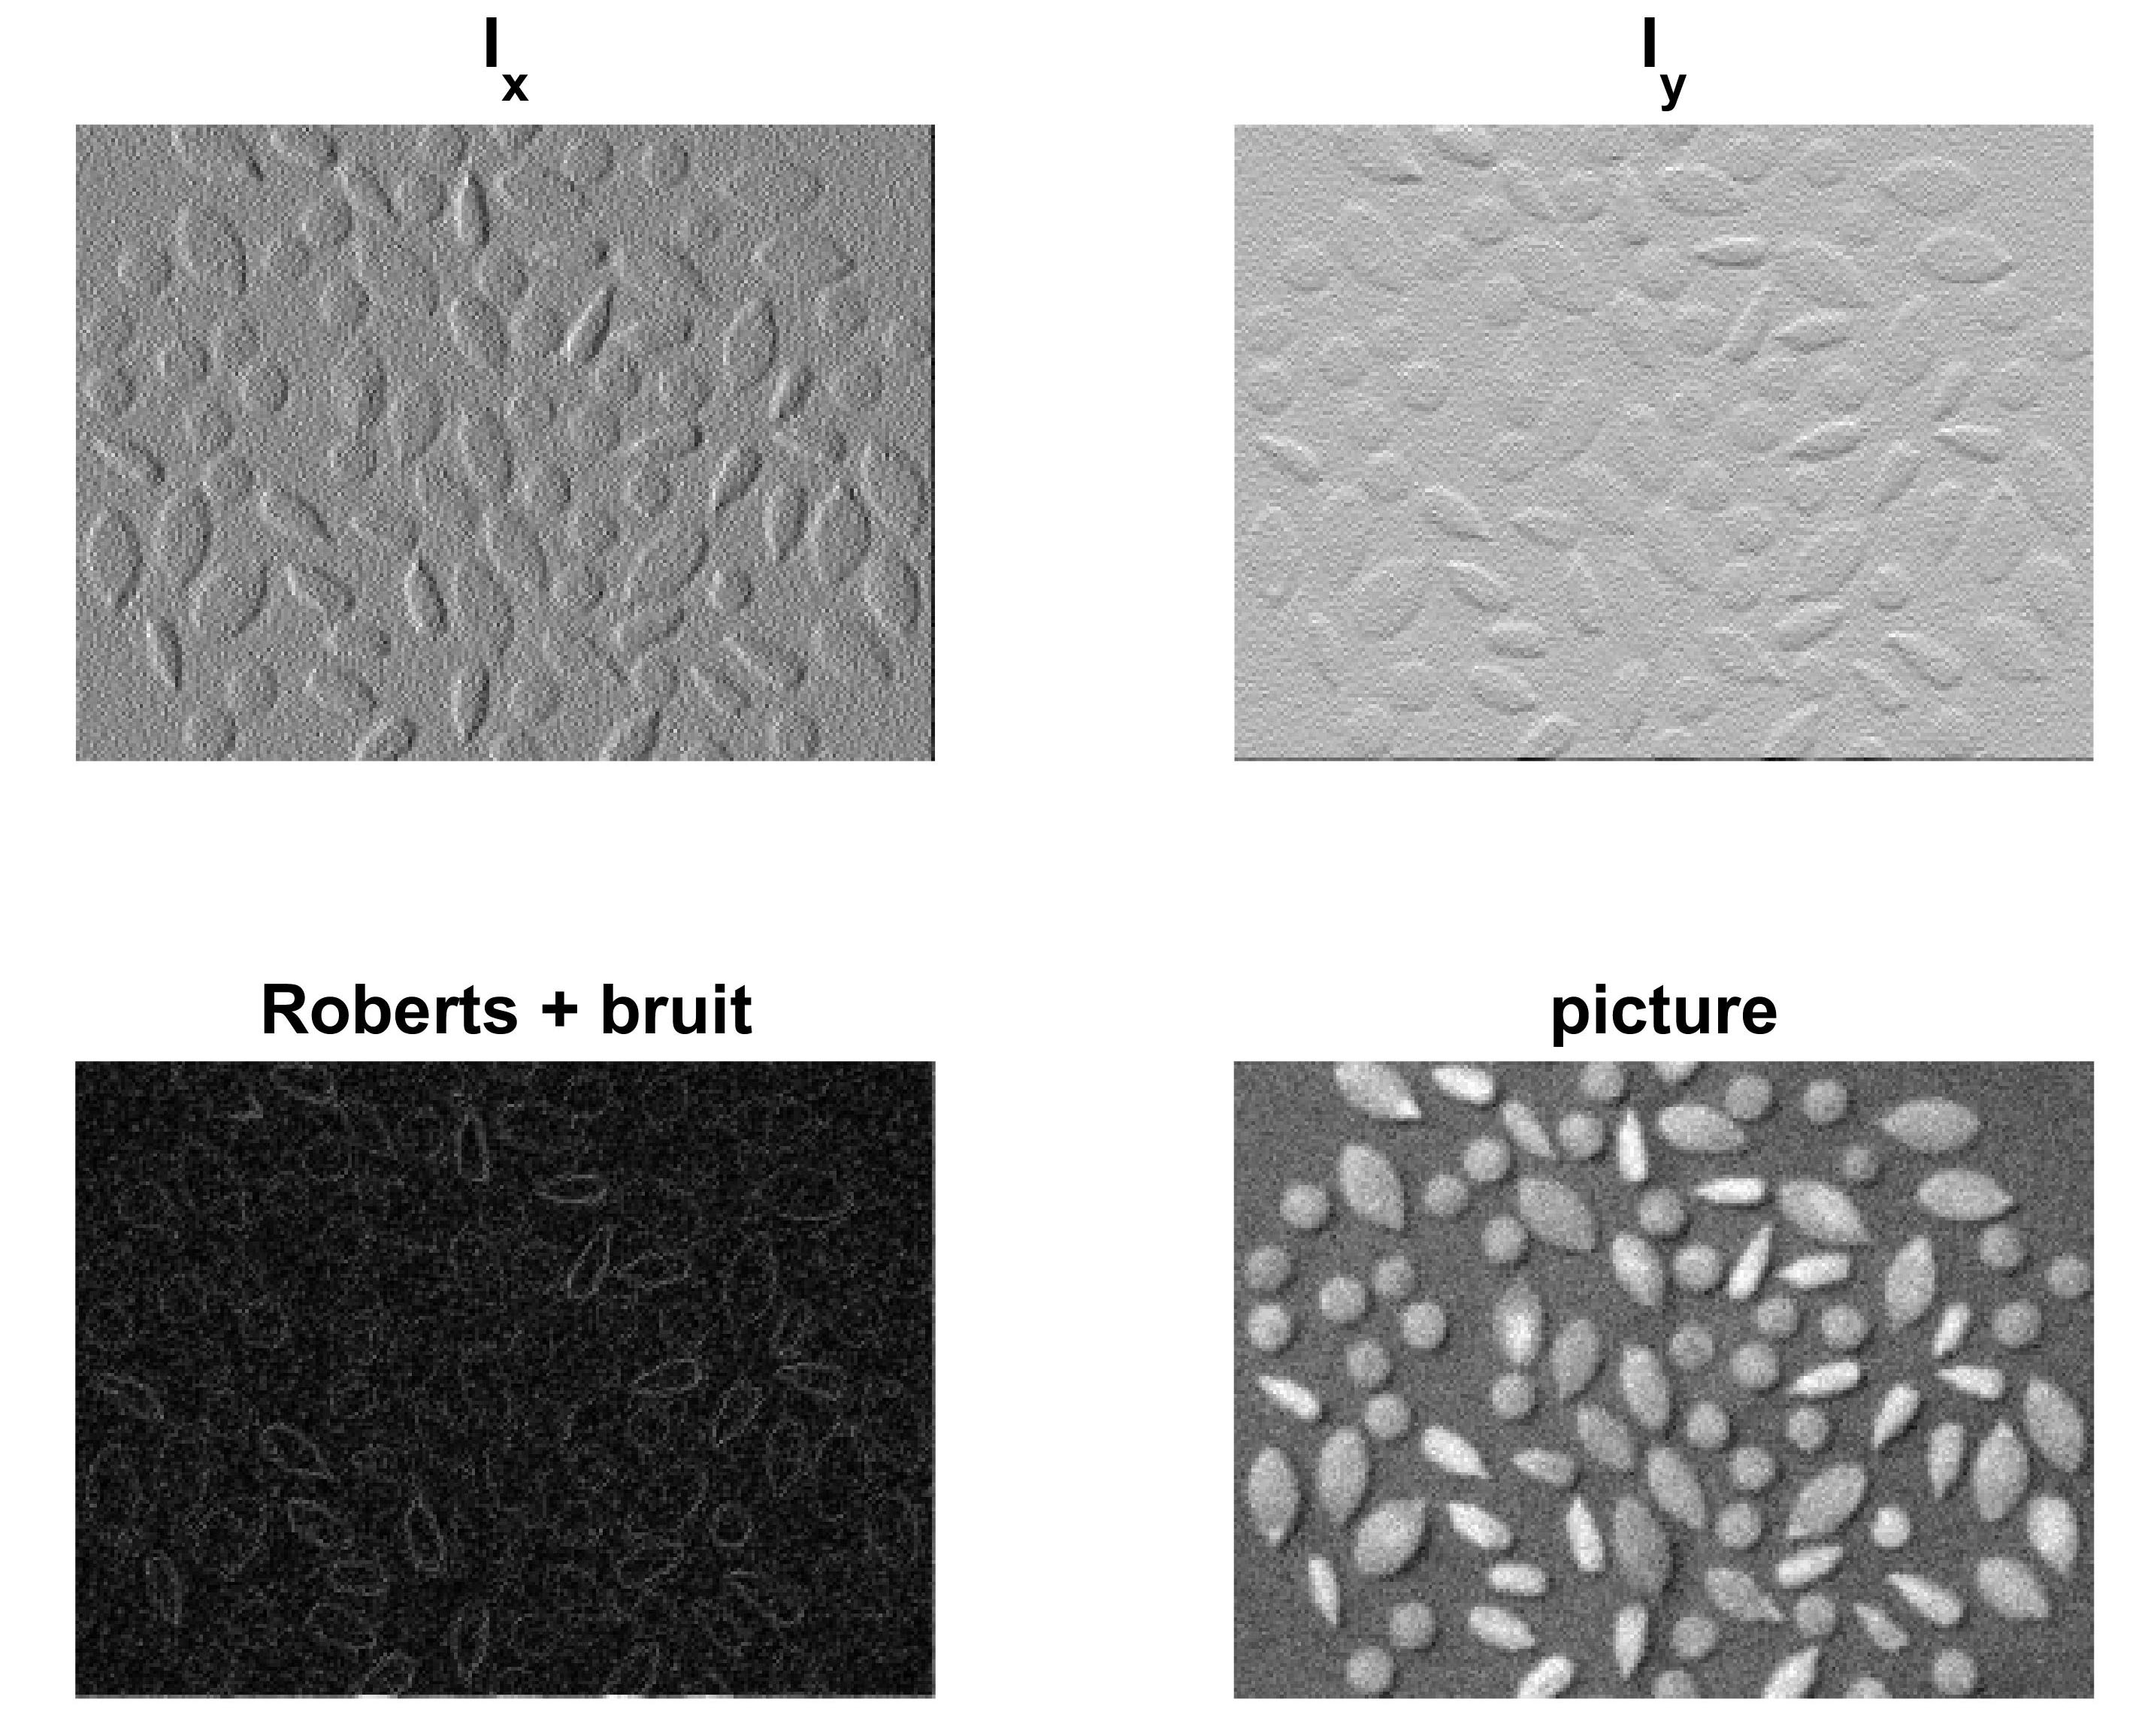
\includegraphics[width=10cm]{bruit_gauss_roberts.jpg}}
\end{center}

	\item Avec le filtre de Sobel :

\begin{center}
\fbox{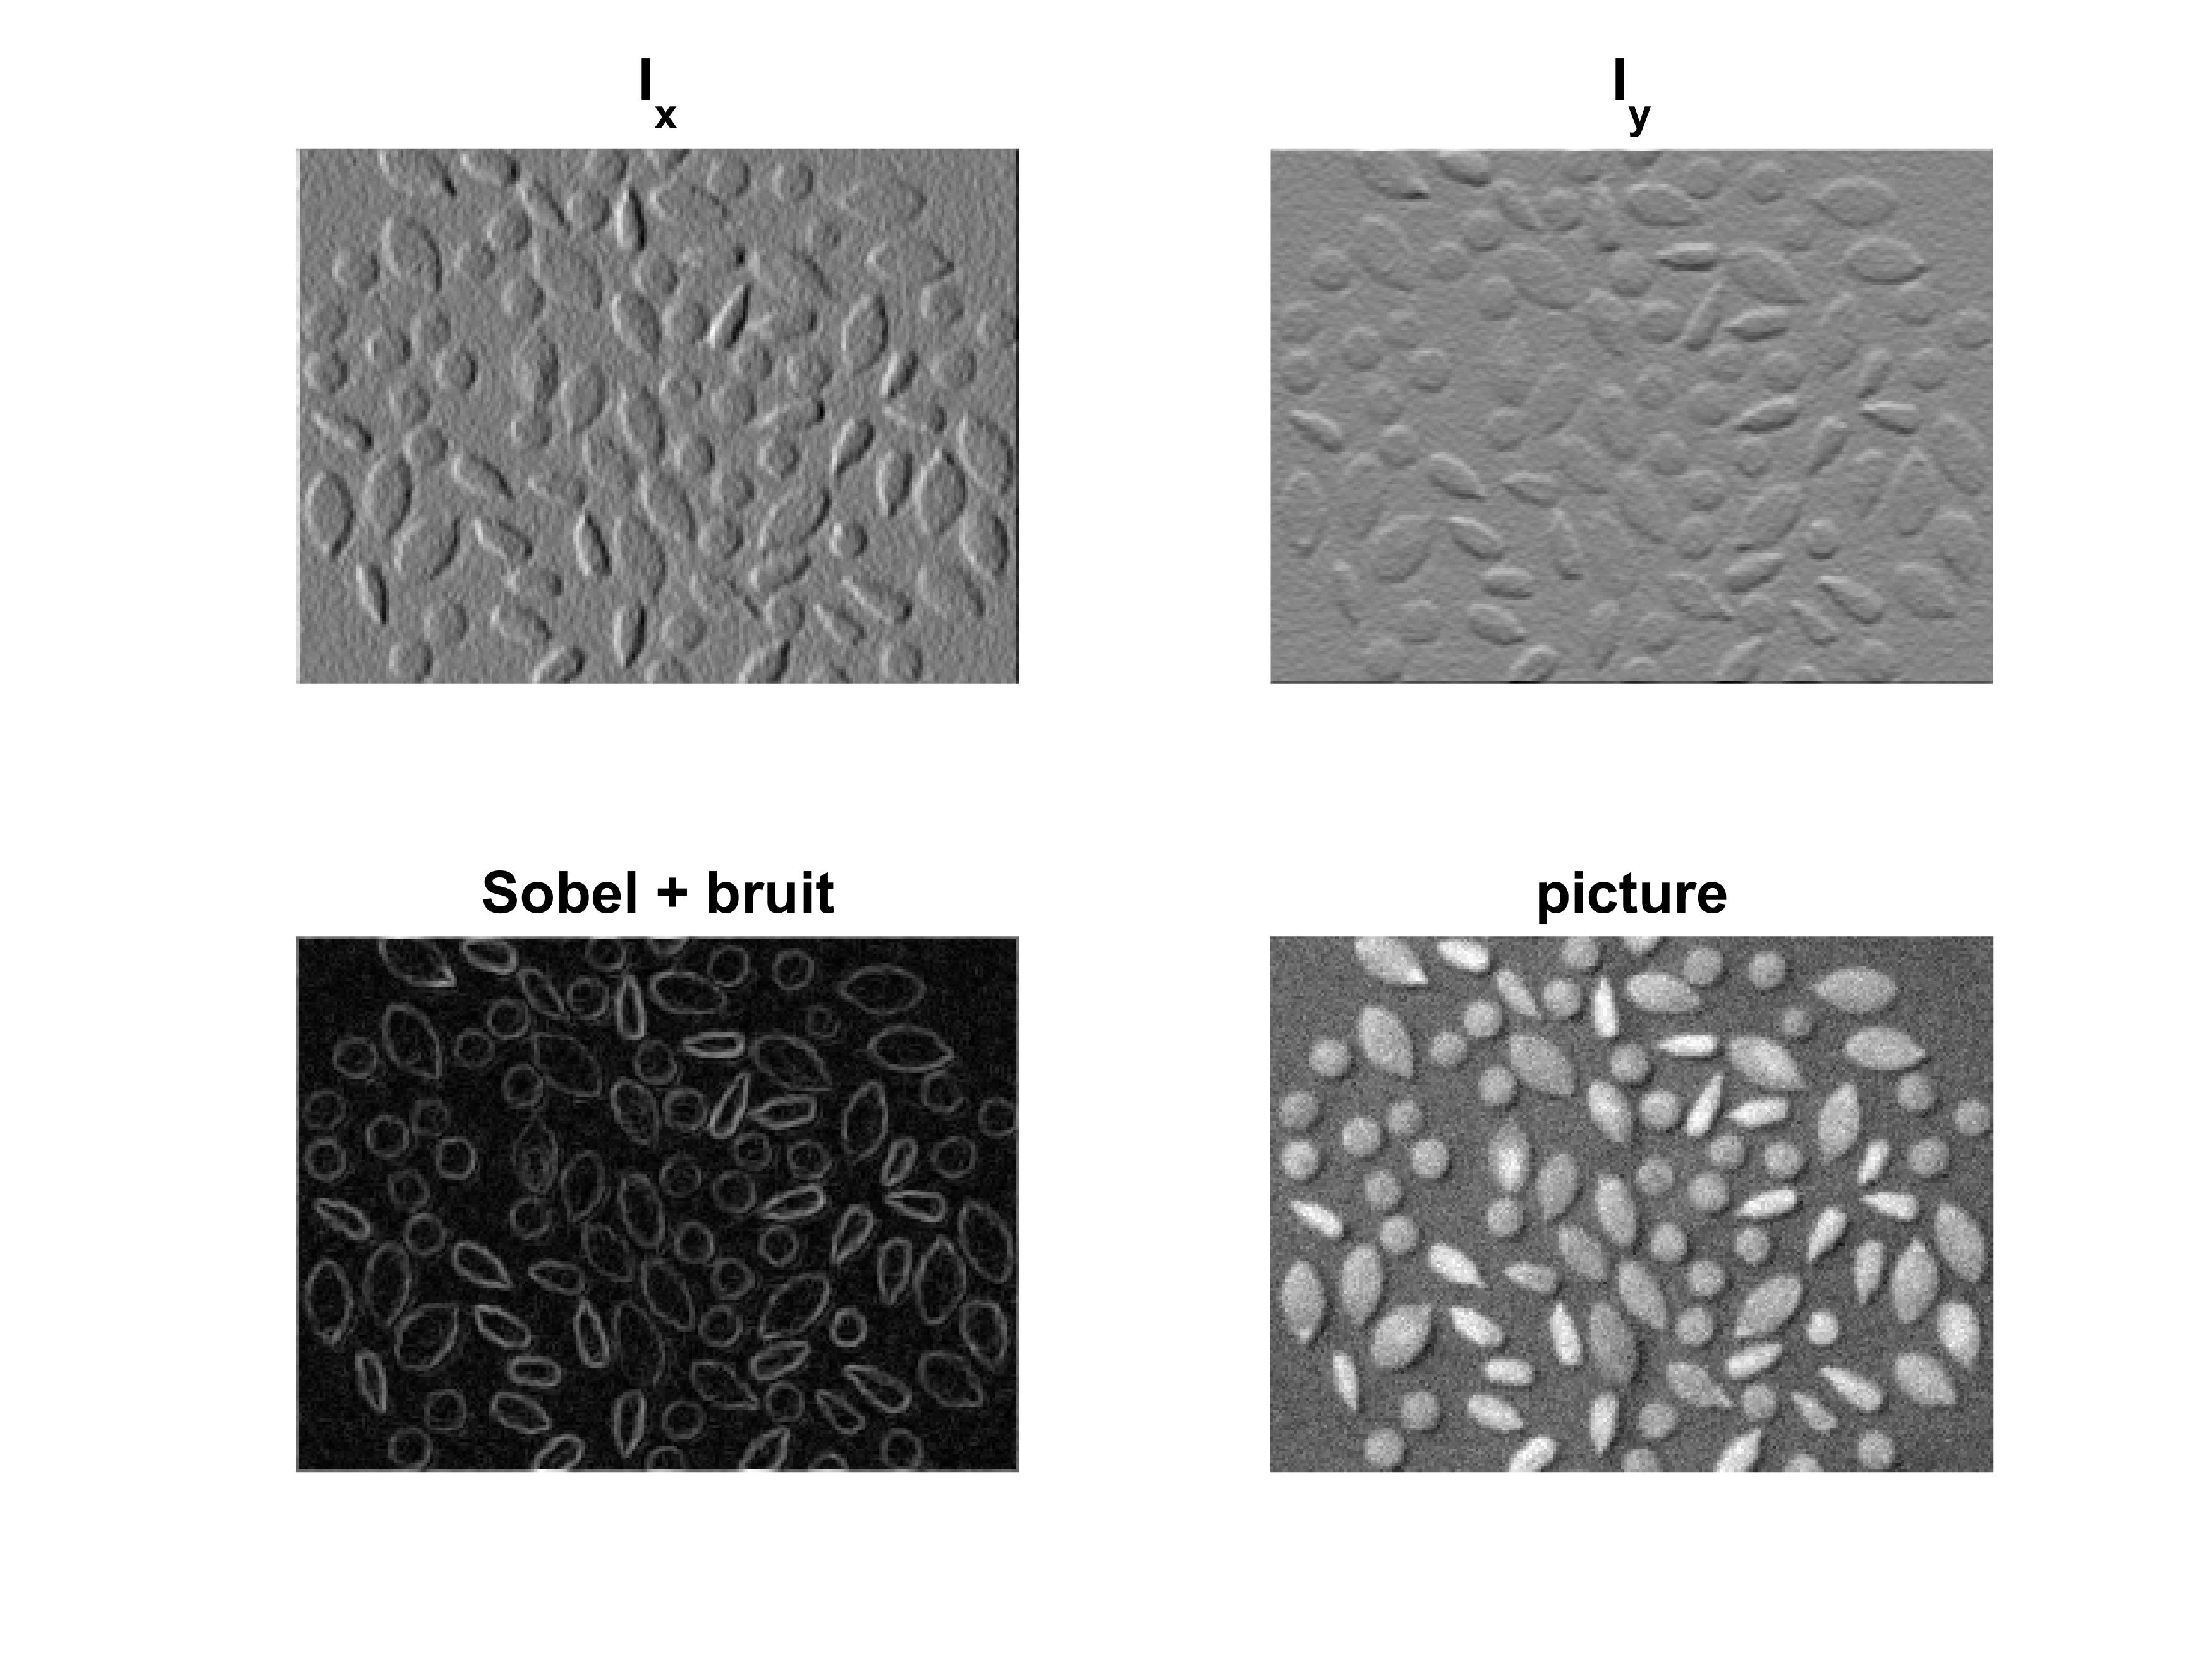
\includegraphics[width=10cm]{bruit_gauss_sobel.jpg}}	
\end{center}

\end{itemize}

On constate que la méthode utilisant le filtre de Roberts n'est vraiment pas efficace dès qu'on a du bruit sur l'image.

En effet, on a du mal à constater correctement les contours des graines.\\

La méthode utilisant le filtre de Sobel est beaucoup plus robuste face au bruit car les contours des graines est assez bien conservé même si on observe légèrement les contours correspondant au bruit dans l'image de la norme.

\section*{3. Recherche des maxima locaux dans la direction du gradient}

\begin{itemize}\renewcommand{\labelitemi}{$\bullet$}
	\item Interpolation au plus proche voisin (nearest)

\begin{center}
\fbox{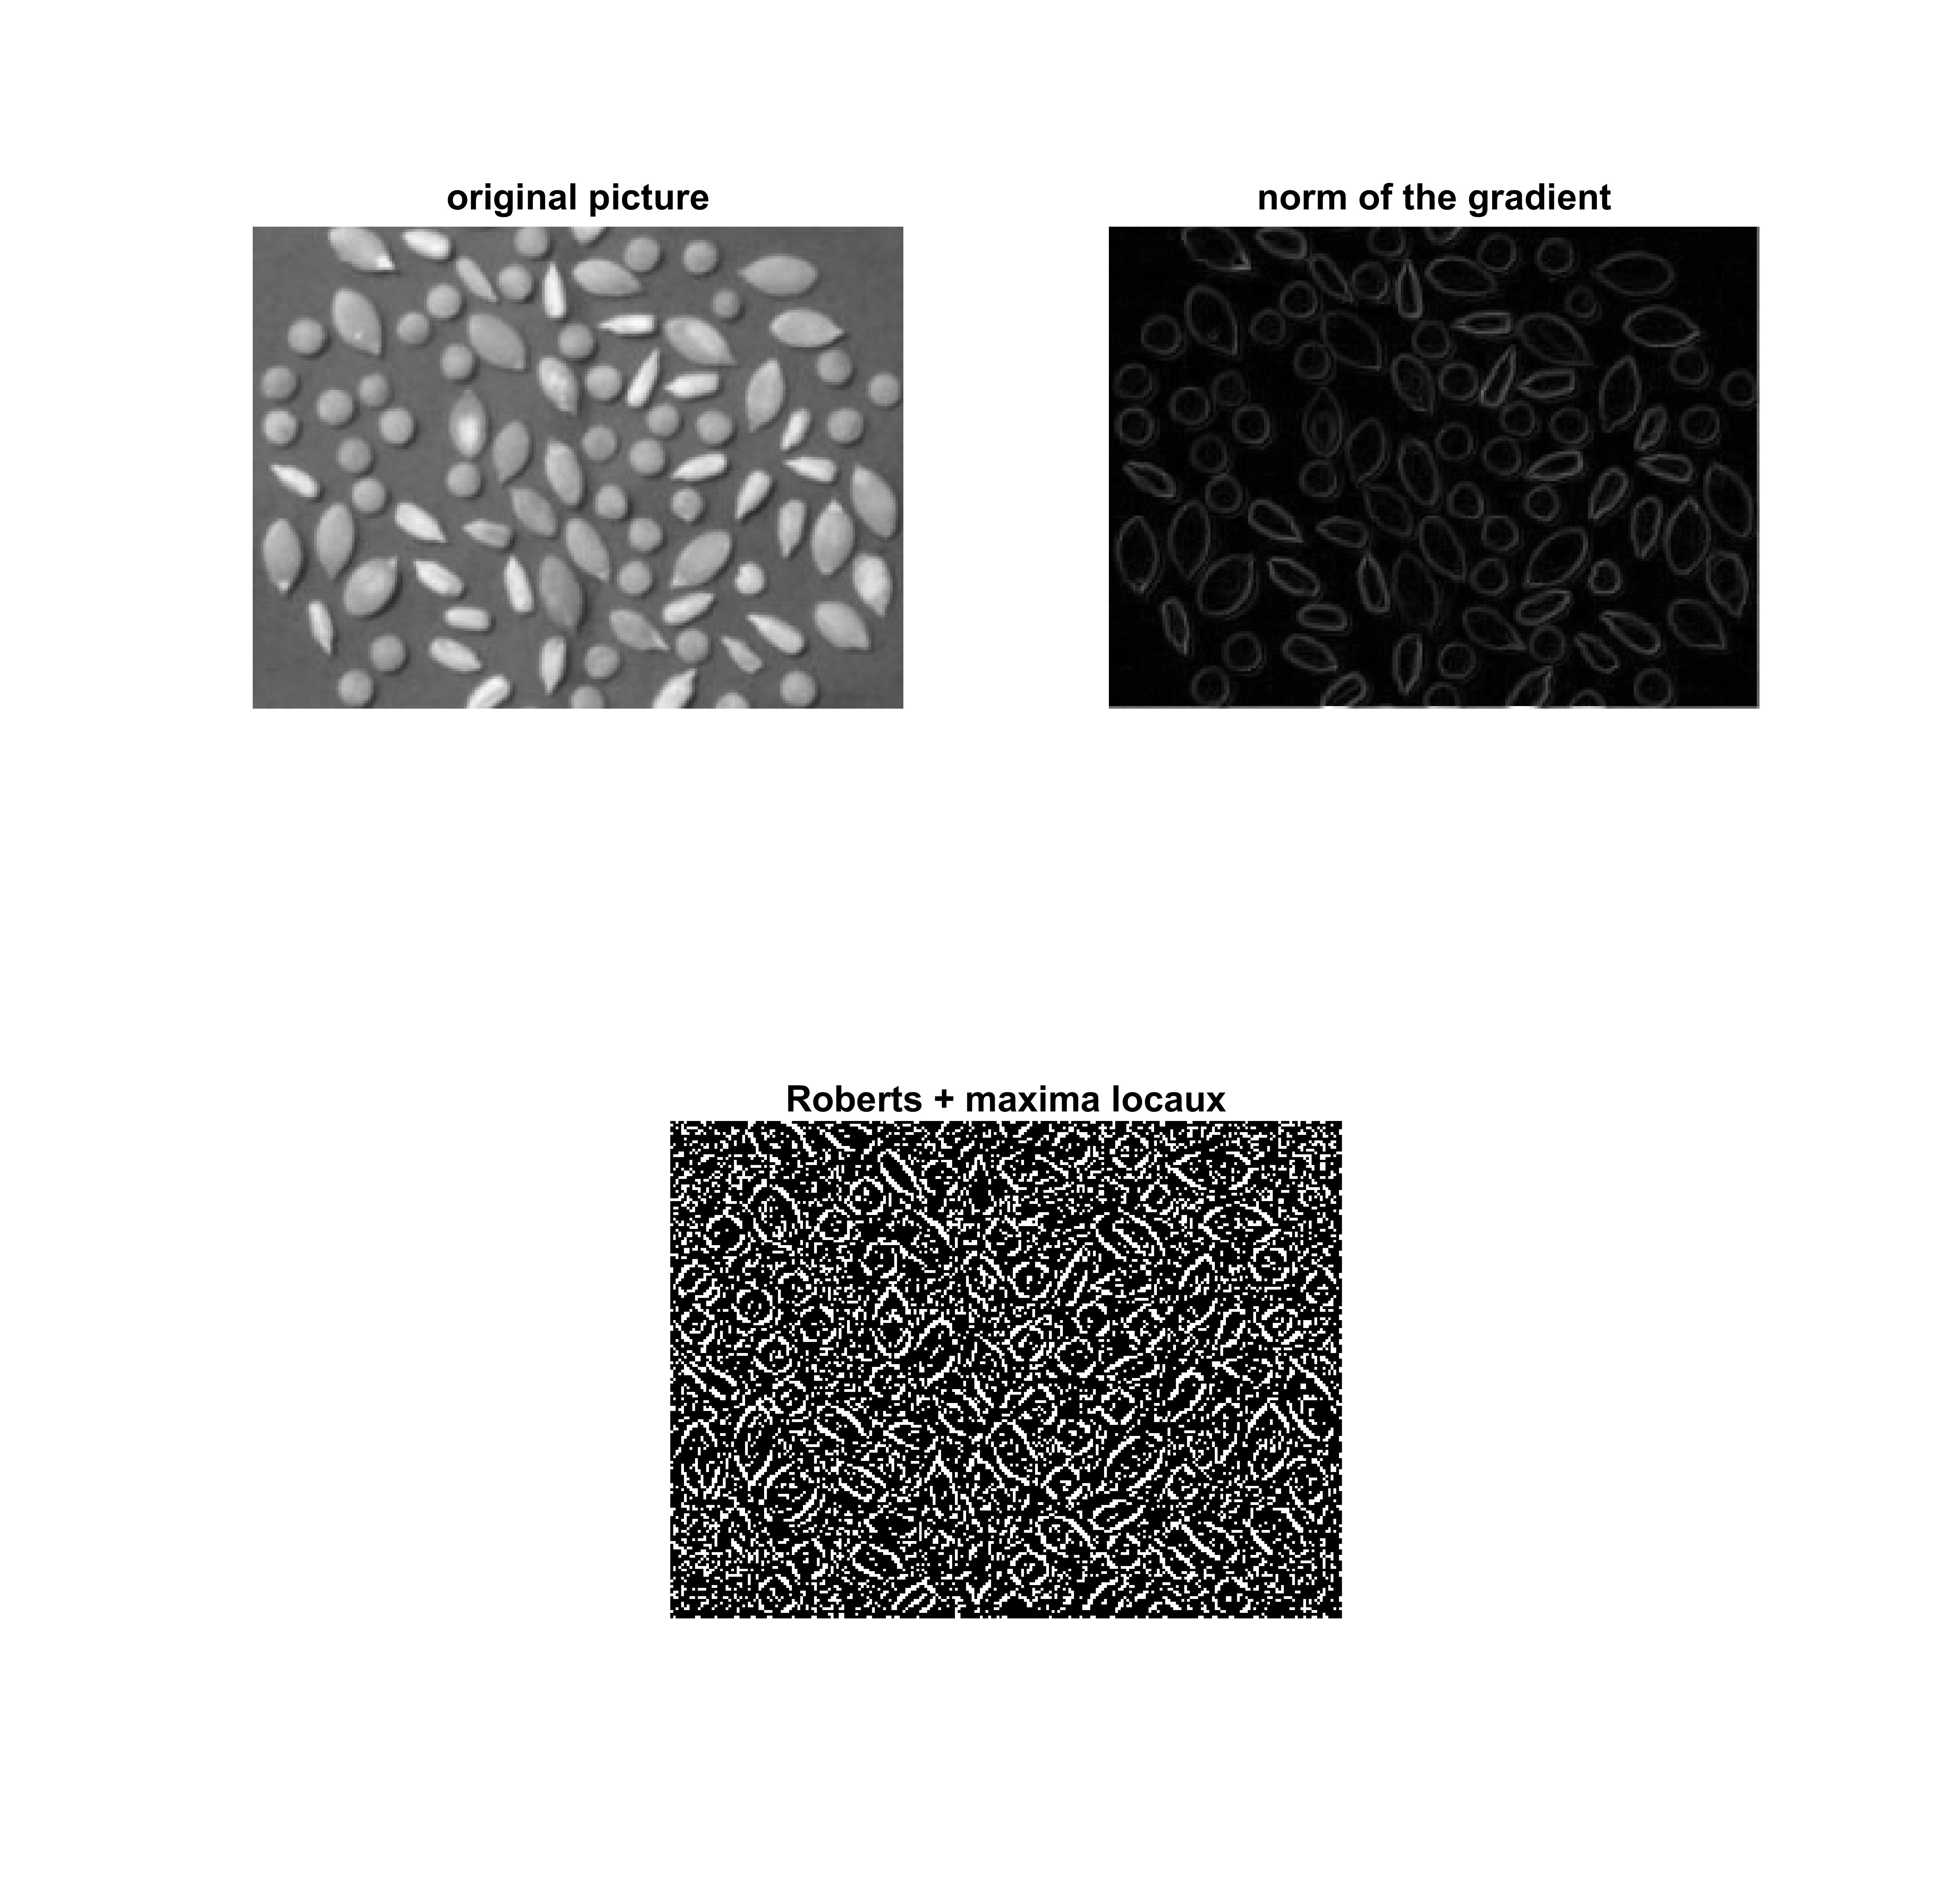
\includegraphics[width=10cm]{roberts_nearest.jpg}}
	
\fbox{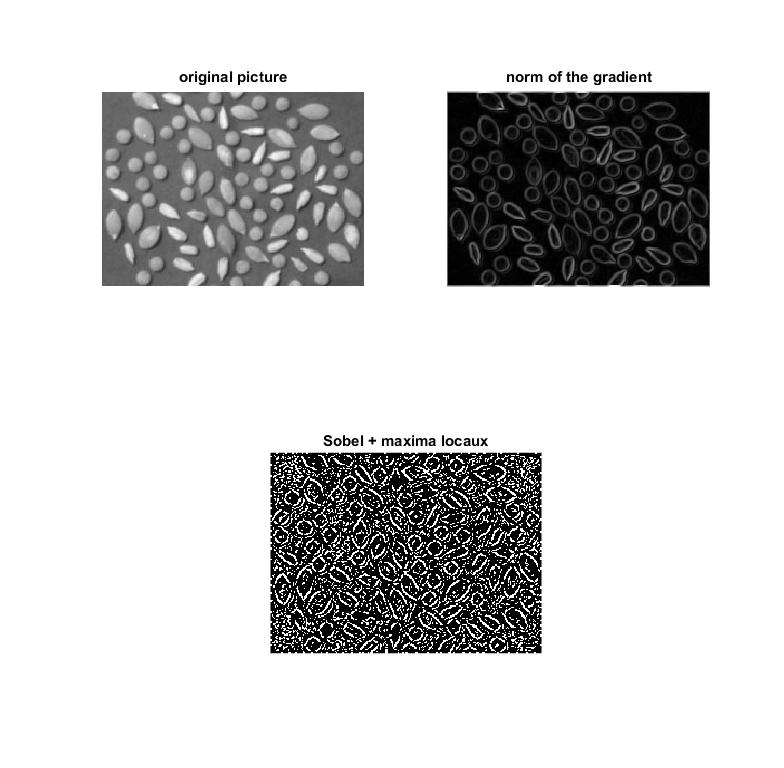
\includegraphics[width=10cm]{sobel_nearest.jpg}}	
\end{center}

	\item Interpolation bilinéaire

\begin{center}
\fbox{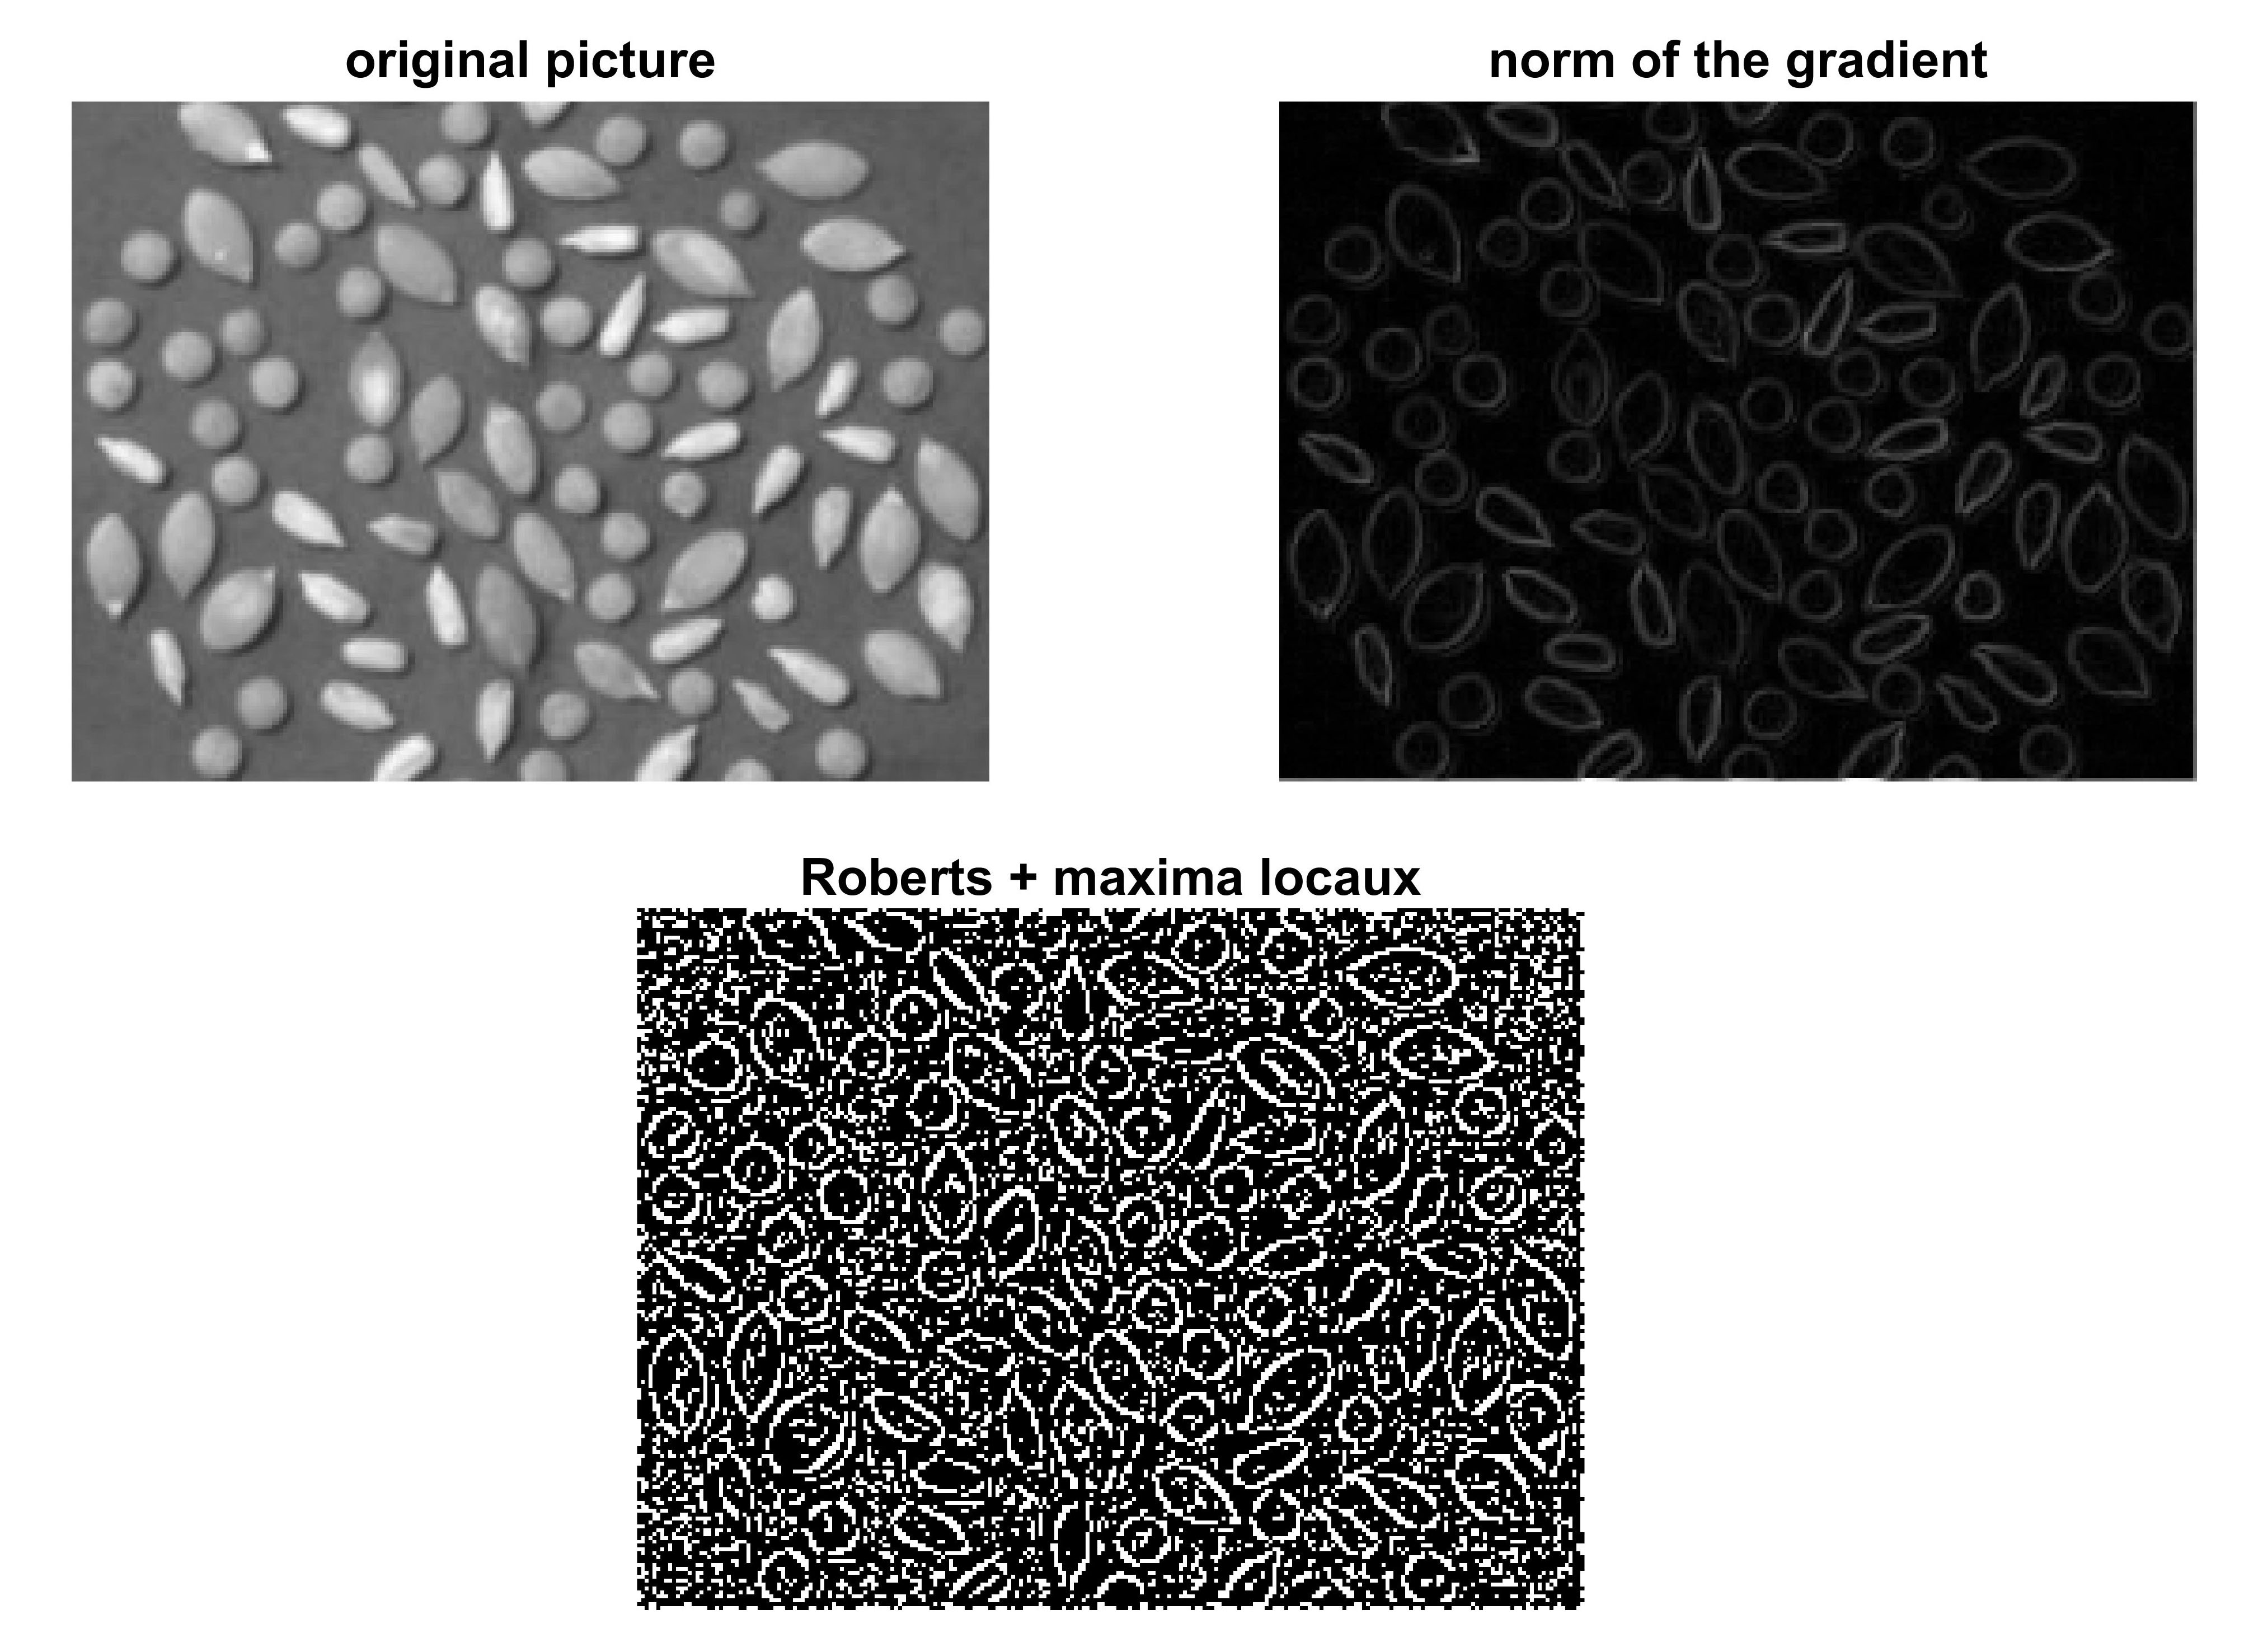
\includegraphics[width=10cm]{roberts_bilinear.jpg}}
	
\fbox{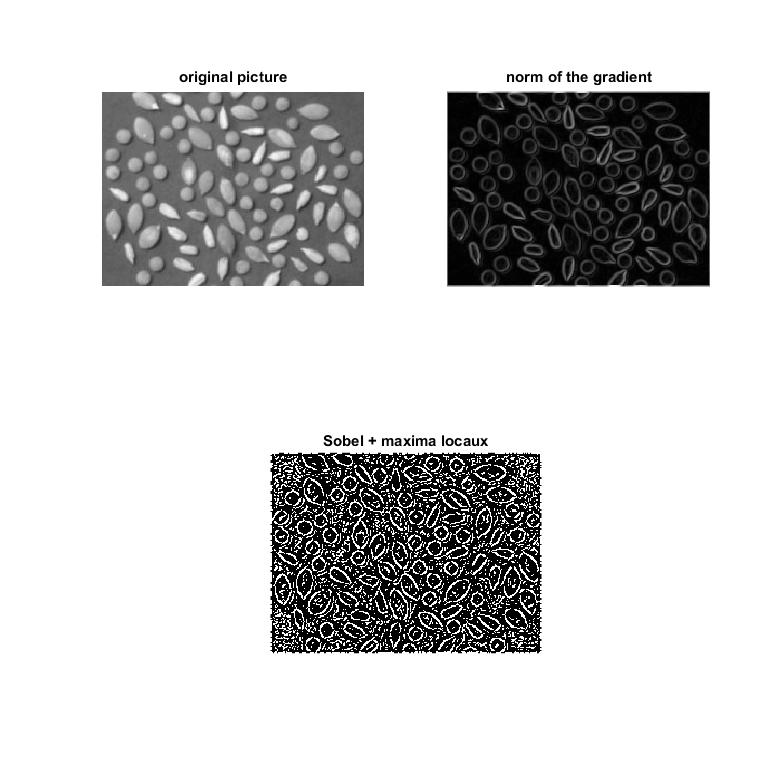
\includegraphics[width=10cm]{sobel_bilinear.jpg}}	
\end{center}

Sobel est encore une fois plus efficace pour rechercher les maxima locaux (en nearest ou bilinéaire).

En bilinéaire, les contours sont globalement plus nets (pour Sobel ou Roberts).		

\end{itemize}

\section*{4. Seuillage et chaînage des points de contour}

\begin{itemize}\renewcommand{\labelitemi}{$\bullet$}
	\item Fonction "link\_picture" dans MatLab :
	
\begin{lstlisting}
%Passe No 1
for i = 2:N_i-1
    for j = 2:N_j-1
         if is_edges_points(i,j)==1
            v1 = [i, j-1];
            v2 = [i-1, j-1];
            v3 = [i-1, j];
            v4 = [i-1, j+1];
            if edges_points(v1(1,1), v1(1,2)) == 1
                edges_points(i,j) = 1;
            end
            if edges_points(v2(1,1), v2(1,2)) == 1
                edges_points(i,j) = 1;
            end
            if edges_points(v3(1,1), v3(1,2)) == 1
                edges_points(i,j) = 1;
            end 
            if v4(1,1) <= 180 && v4(1,1) > 0 && v4(1,2) > 0 && v4(1,2) <= 243
                if edges_points(v4(1,1), v4(1,2)) == 1 
                    edges_points(i,j) = 1;
                end
            end
         end
    end
end

%Passe No 2
for j = N_j-1:-1:2
    for i=2 :N_i-1
         if is_edges_points(i,j)==1
            v1 = [i-1, j];
            v2 = [i-1, j+1];
            v3 = [i, j+1];
            v4 = [i+1, j+1];
            if edges_points(v1(1,1), v1(1,2)) == 1
                edges_points(i,j) = 1;
            end
            
            if edges_points(v2(1,1), v2(1,2)) == 1
                edges_points(i,j) = 1;
            end
            
            if edges_points(v3(1,1), v3(1,2)) == 1
                edges_points(i,j) = 1;
            end
            
            if v4(1,1) <= 180 && v4(1,1) > 0 && v4(1,2) > 0 && v4(1,2) <= 243
               if edges_points(v4(1,1), v4(1,2)) == 1
                   edges_points(i, j) = 1;
               end
            end
         end
    end
end

%Passe No 3
for i =N_i-1:-1:2
    for j=N_j-1:-1 :2
         if is_edges_points(i,j)==1
            v1 = [i, j+1];
            v2 = [i+1, j+1];
            v3 = [i+1, j];
            v4 = [i+1, j-1];
                
            if edges_points(v1(1,1), v1(1,2)) == 1
                edges_points(i,j) = 1;
            end
            
            if edges_points(v2(1,1), v2(1,2)) == 1
                edges_points(i,j) = 1;
            end
            
            if edges_points(v3(1,1), v3(1,2)) == 1
                edges_points(i,j) = 1;
            end
            
            if v4(1,1) <= 180 && v4(1,1) > 0 && v4(1,2) > 0 && v4(1,2) <= 243
               if edges_points(v4(1,1), v4(1,2)) == 1
                   edges_points(i, j) = 1;
               end
            end
         end
    end
end

%Passe No 4
for j =2   :N_j-1
    for i=N_i-1:-1 :2
         if is_edges_points(i,j)==1
            v1 = [i+1, j];
            v2 = [i+1, j-1];
            v3 = [i, j-1];
            v4 = [i-1, j-1];

            if edges_points(v1(1,1), v1(1,2)) == 1
                edges_points(i,j) = 1;
            end
            
            if edges_points(v2(1,1), v2(1,2)) == 1
                edges_points(i,j) = 1;
            end
            
            if edges_points(v3(1,1), v3(1,2)) == 1
                edges_points(i,j) = 1;
            end
            
            if v4(1,1) <= 180 && v4(1,1) > 0 && v4(1,2) > 0 && v4(1,2) <= 243
               if edges_points(v4(1,1), v4(1,2)) == 1
                   edges_points(i, j) = 1;
               end
            end
         end
    end
end
\end{lstlisting}
\end{itemize}

\section*{5. Exécution de la chaîne complète de détection de contours}

\begin{itemize}[leftmargin=*]\renewcommand{\labelitemi}{$\bullet$}
	\item Contours obtenus
	\begin{itemize}[leftmargin=*]
		\item Méthode de Roberts
		
\begin{minipage}[c]{0.46\linewidth}				
	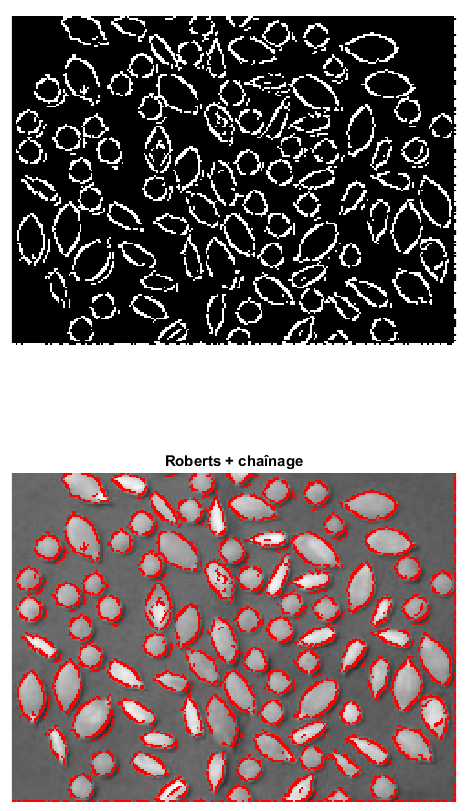
\includegraphics[width=8cm]{Roberts_link.png}
	\captionof{figure}{Chaînage sans bruit}
\end{minipage}\hfill
\begin{minipage}[c]{0.46\linewidth}
	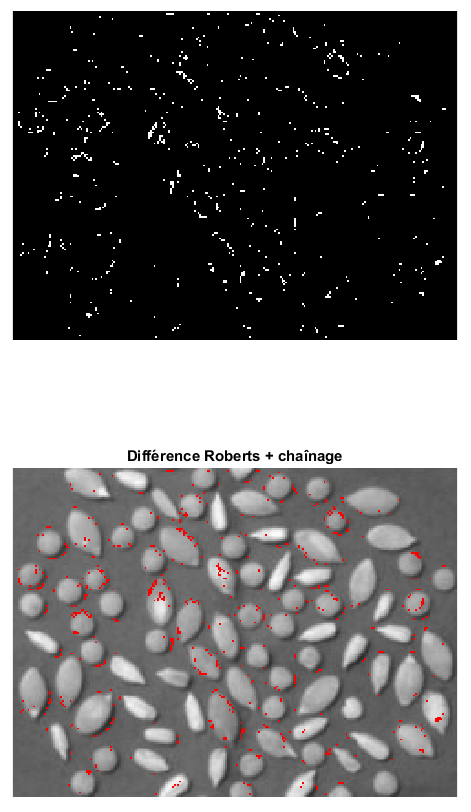
\includegraphics[width=8cm]{Diff_Roberts_link.png}
	\captionof{figure}{Chaînes rajoutées (sans bruit)}
\end{minipage}\hfill

\begin{minipage}[c]{0.46\linewidth}		
	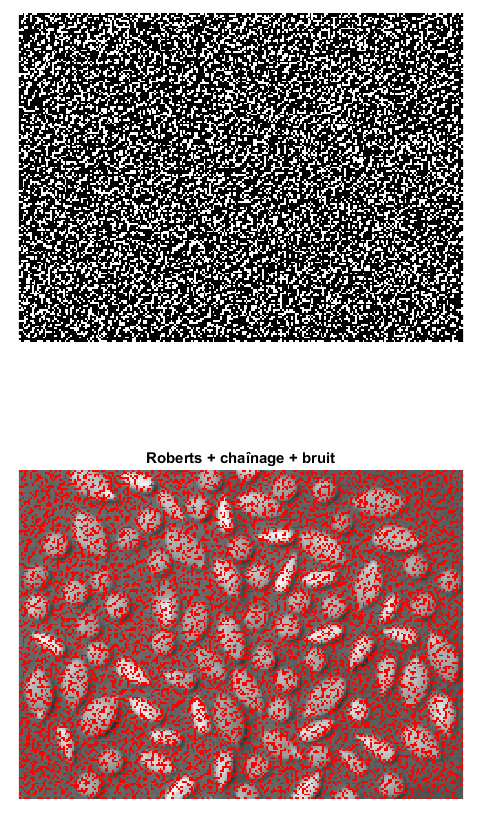
\includegraphics[width=8cm]{Roberts_link_noise5.png}
	\captionof{figure}{Chaînage avec rsb=5db}
\end{minipage}\hfill
\begin{minipage}[c]{0.46\linewidth}
	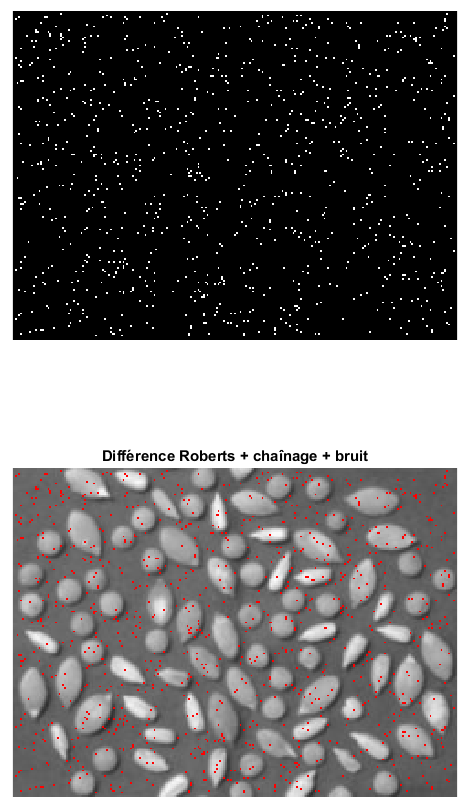
\includegraphics[width=8cm]{Diff_Roberts_link_noise5.png}
	\captionof{figure}{Chaînes rajoutées (rsb=5db)}
\end{minipage}\hfill

\begin{minipage}[c]{0.46\linewidth}		
	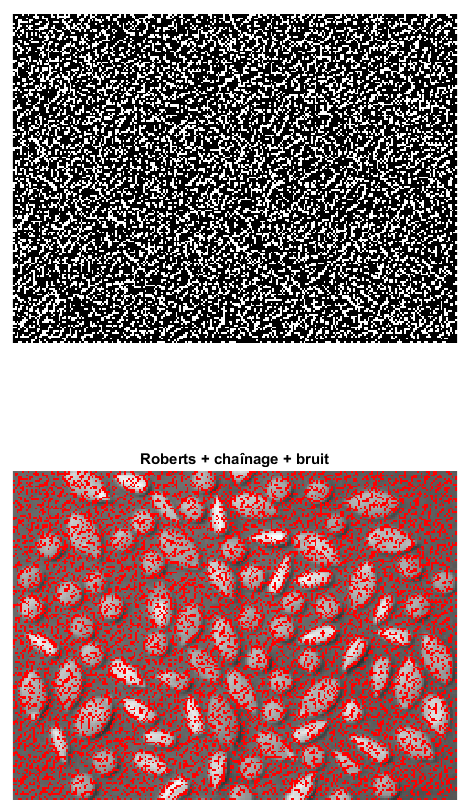
\includegraphics[width=8cm]{Roberts_link_noise10.png}
	\captionof{figure}{Chaînage avec rsb=10db}
\end{minipage}\hfill
\begin{minipage}[c]{0.46\linewidth}
	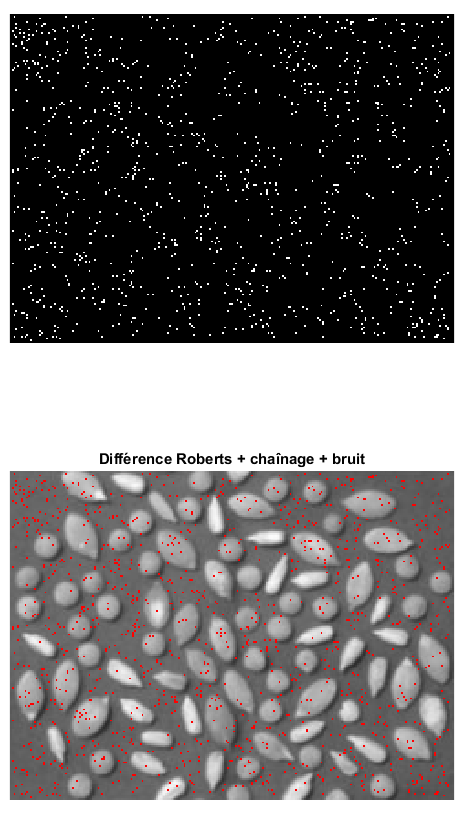
\includegraphics[width=8cm]{Diff_Roberts_link_noise10.png}
	\captionof{figure}{Chaînes rajoutées (rsb=10db)}
\end{minipage}\hfill

\begin{minipage}[c]{0.46\linewidth}		
	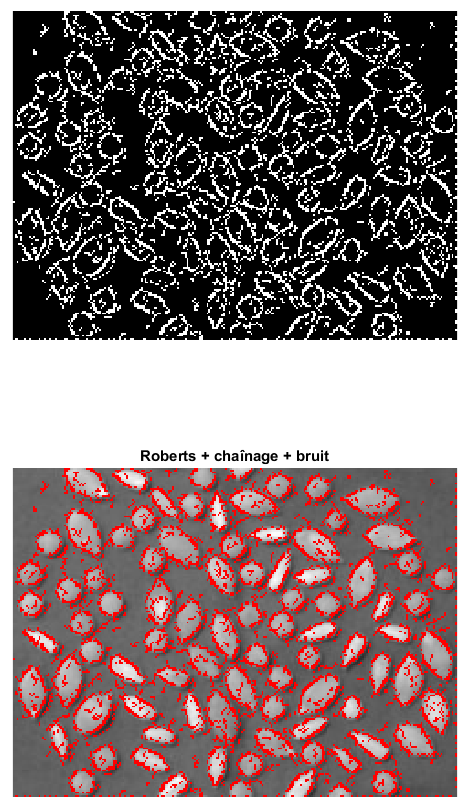
\includegraphics[width=8cm]{Roberts_link_noise20.png}
	\captionof{figure}{Chaînage avec rsb=20db}
\end{minipage}\hfill
\begin{minipage}[c]{0.46\linewidth}
	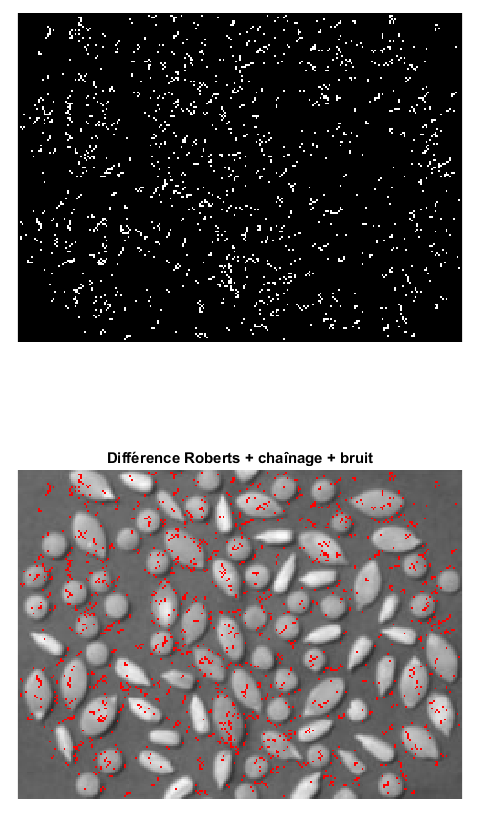
\includegraphics[width=8cm]{Diff_Roberts_link_noise20.png}
	\captionof{figure}{Chaînes rajoutées (rsb=20db)}	
\end{minipage}\hfill
	
		\item Méthode de Sobel
		
\begin{minipage}[c]{0.46\linewidth}		
	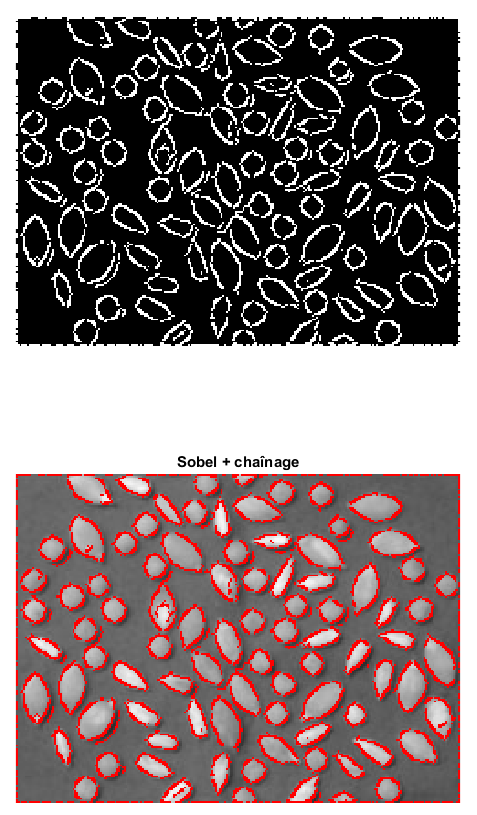
\includegraphics[width=8cm]{Sobel_link.png}
	\captionof{figure}{Chaînage sans bruit}
\end{minipage}\hfill
\begin{minipage}[c]{0.46\linewidth}
	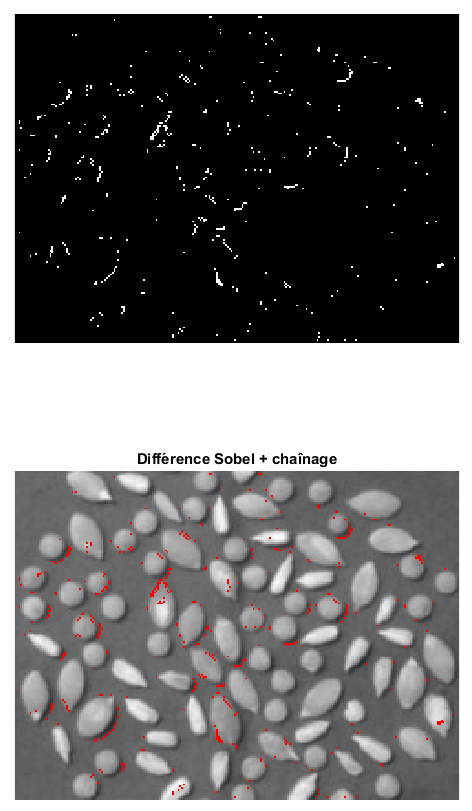
\includegraphics[width=8cm]{Diff_Sobel_link.png}
	\captionof{figure}{Chaînes rajoutées (sans bruit)}
\end{minipage}\hfill

\begin{minipage}[c]{0.46\linewidth}		
	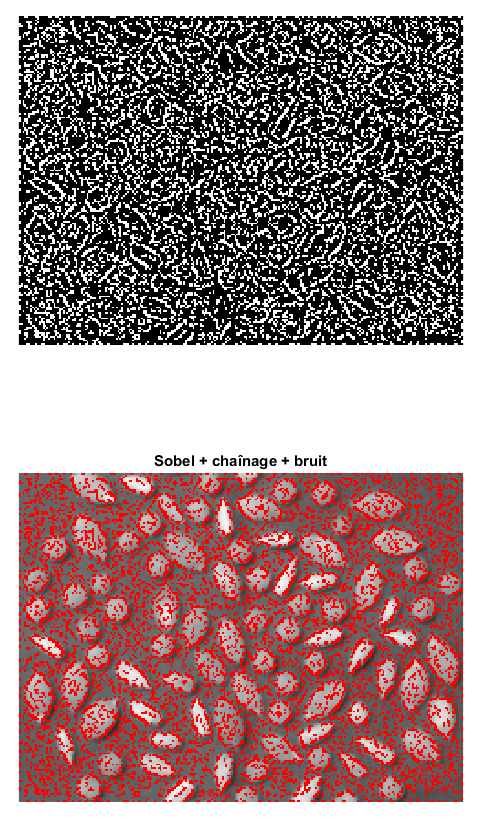
\includegraphics[width=8cm]{Sobel_link_noise5.png}
	\captionof{figure}{Chaînage avec rsb=5db}
\end{minipage}\hfill
\begin{minipage}[c]{0.46\linewidth}
	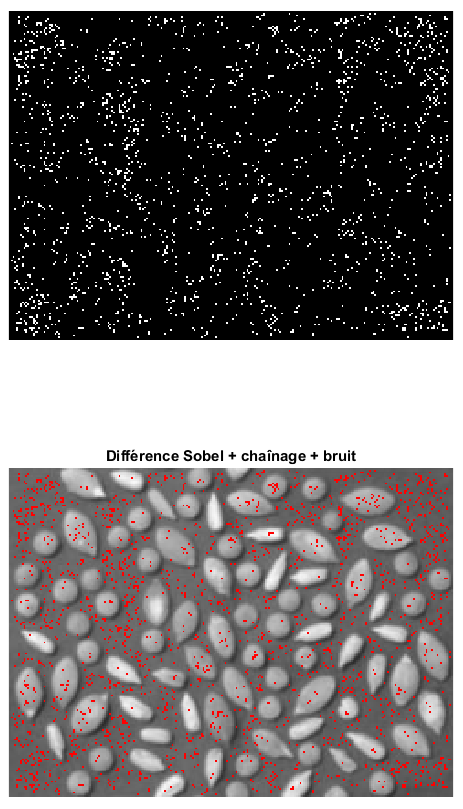
\includegraphics[width=8cm]{Diff_Sobel_link_noise5.png}
	\captionof{figure}{Chaînes rajoutées (rsb=5db)}
\end{minipage}\hfill

\begin{minipage}[c]{0.46\linewidth}		
	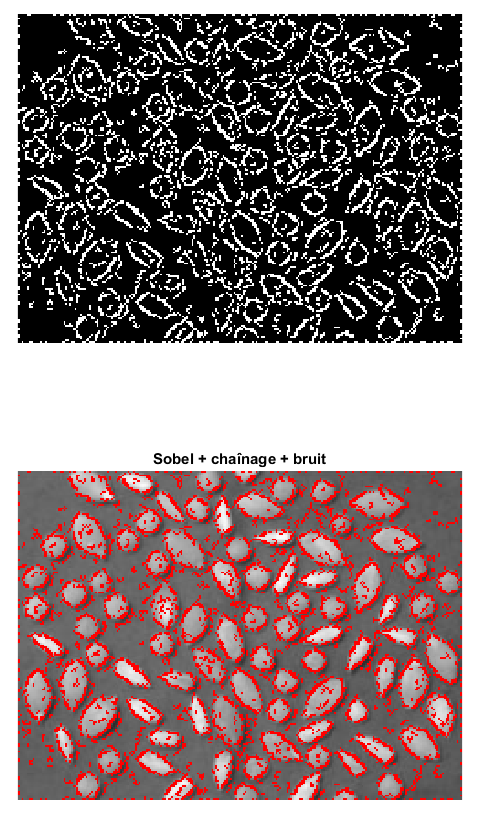
\includegraphics[width=8cm]{Sobel_link_noise10.png}
	\captionof{figure}{Chaînage avec rsb=10db}
\end{minipage}\hfill
\begin{minipage}[c]{0.46\linewidth}
	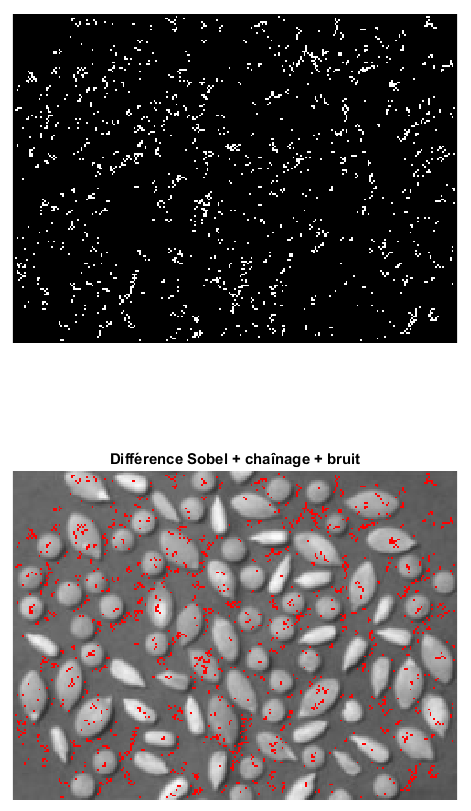
\includegraphics[width=8cm]{Diff_Sobel_link_noise10.png}
	\captionof{figure}{Chaînes rajoutées (rsb=10db)}
\end{minipage}\hfill

\begin{minipage}[c]{0.46\linewidth}		
	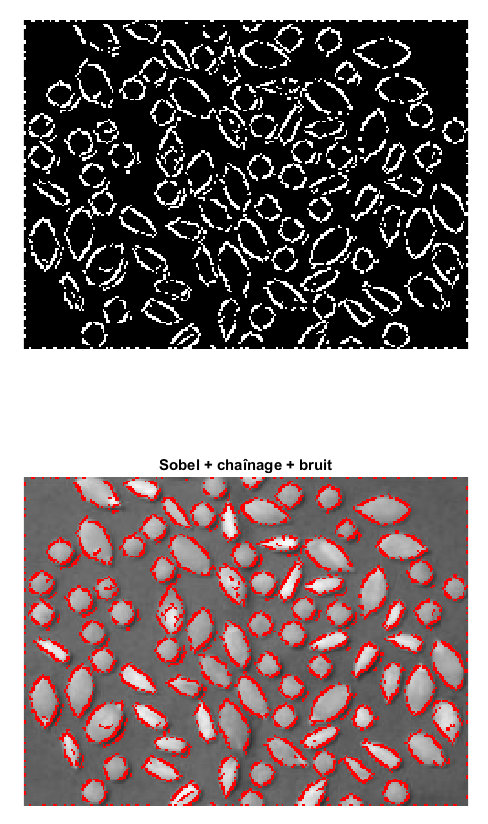
\includegraphics[width=8cm]{Sobel_link_noise20.png}
	\captionof{figure}{Chaînage avec rsb=20db}
\end{minipage}\hfill
\begin{minipage}[c]{0.46\linewidth}
	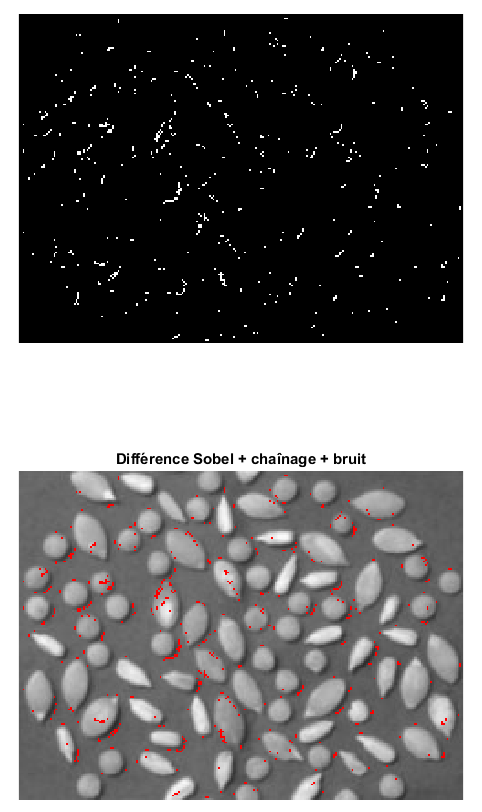
\includegraphics[width=8cm]{Diff_Sobel_link_noise20.png}
	\captionof{figure}{Chaînes rajoutées (rsb=20db)}	
\end{minipage}\hfill
	\end{itemize}
	
	\item Lorsque l'on fait varier la valeur de d, on remarque un changement au niveau des contours.

En effet, lorsqu'on augmente la valeur de d, les contours détectés vont être plus épais mais moins contigus.

Si on rapproche la valeur de d de 1, les contours détectés sont donc plus fins mais parfois pas complets (on observe des trous dans les contours des graines).

Au niveau du bruit, on constate toujours que la méthode de Sobel est plus robuste même si à partir d'un rsb de 5db la détection des contours est beaucoup moins efficace.


\end{itemize}

\end{document}